\chapter{Parte II}

Nella seconda parte delle progetto abbiamo sviluppato una rete neurale che non si limita ad approssimare la formula \ref{eqn:formula} ma tiene conto anche delle diffenze percettive dell'occhio umano. L'equazione infatti è imprecisa per certe zone dello spazio L*a*b e pertanto l'output della rete neurale precedente va corretto. Per fare ciò è necessario passare dallo spazio di colore CIE L*a*b allo spazio di colore CIE L*C*h ed infine definire delle regole di inferenza per un sistema fuzzy di tipo Mamdani.
Ricordiamo gli intervalli delle coordinate nello spazio L*C*h.
\begin{itemize}
	\item \textit{Lightness (L\textsuperscript{*})} Range [0, 100]
	\item \textit{Hue (h)} Range  [0, 360\textdegree] 
    \item \textit{Chroma (C\textsuperscript{*})} Il range dipende dal valore L\textsuperscript{*}. \(C\textsubscript{max}= 127\) quando 
    \(L\textsuperscript{*}=50\) cioè quando si è al centro dell'ellissoide descritto dall spazio L*C*h mentre è \(C\textsuperscript{*}=0\) quando \(L\textsuperscript{*}=0\) oppure \(L\textsuperscript{*}=100\). La relazione tra \(L\textsuperscript{*}\) e \(C\textsuperscript{*}\) quindi si può descrivere come un ellisse.
    	\begin{equation}\label{eqn:ellipse}
       		\frac{C^2}{127^2} + \frac{(L-50)^2}{50^2} = 1
       	\end{equation}
    Quindi \({C^{'}}\textsubscript{max}\) si può calcolare come
    	\begin{equation}\label{eqn:c_primo_max}
    		{C^{'}}\textsubscript{max} = 127\sqrt{1 - \frac{(L-50)^2}{50^2}}
    	\end{equation}
    Pertanto definiamo 
         \begin{equation}\label{eqn:cperc}
       		c\% = 100\frac{C}{ {C^{'}}\textsubscript{max}}
       	\end{equation}
    Il range di c\% è [0, 100] ed è questo ultimo valore che useremo per le regole di inferenza.
\end{itemize}

\begin{figure}[!ht]
\begin{center}
	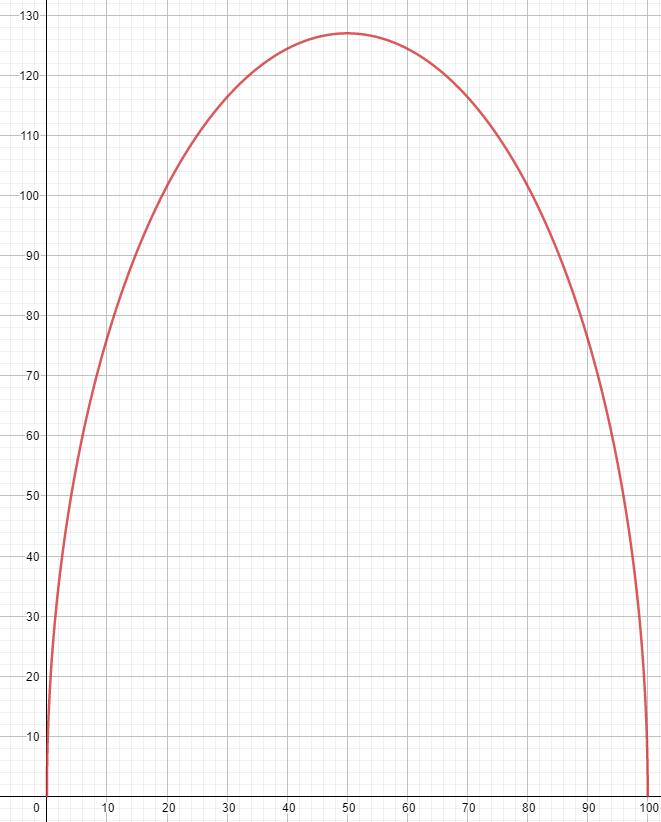
\includegraphics[scale=0.5]{images/geogebra-export.png}
\end{center}
\caption{Grafico del \({C^{'}}_{max}\) al variare di L}
\end{figure}

Le funzioni di membership e le regole della rete fuzzy sono state progettate sulla base della percezione delle differenze delle coppie, analizzando varie aree dello spazio dei colori. Abbiamo notato che, a parità di DeltaE, la differenza delle coppie selezionate può essere percepita diversamente. Per questo motivo abbiamo individuato una serie di zone dello spazio LCh nella quale la percezione è differente da quella evidenziata dal DeltaE.

\paragraph{Colori Insaturi} I colori poco saturi si distinguono con più difficoltà.
\paragraph{Colori Non Luminosi} I colori poco luminosi, similmente a quelli insaturi, non sono facilmente distinguibili.
\paragraph{Zona colori Arancione} I colori tendenti all'arancione sono più distinguibili.
\paragraph{Zona colori Giallo/Verde/Blu} I colori tendenti al giallo, al verde o al blu non sono facilmente distinguibili.

\section{Funzioni di Membership}
Per identificare le zone elencate abbiamo modellato gli ingressi in base al:
\begin{itemize}
	\item il colore (blue, yellow, green, ...)
	\item il livello di saturazione (low/high)
	\item il livello di luminosità (low/mid/high)
	\item il DeltaE dal punto di vista di un osservatore
	\item infine, per l'output, il DeltaE corretto, similmente al DeltaE in ingresso
\end{itemize}
Per quanto riguarda il DeltaE e il DeltaE Corretto ci siamo basati sulla differenza percepita dall'osservatore, identificando le seguenti funzioni di membership:

\begin{itemize}
	\item \( 0 < \Delta E < 1\) \textbf{no-diff}: l'osservatore non percepisce differenze;
	\item \( 1 < \Delta E < 2\) \textbf{exp-diff}: solo osservatori con esperienza riescono a notare una differenza;
	\item \( 2 < \Delta E < 3.5\) \textbf{unexp-diff}: osservatore senza esperienza riescono a notare la differenza;
	\item \( 3.5 < \Delta E < 5\) \textbf{clear-diff}: i colori sono facilmente distinguibili;
	\item \( \Delta E \geq 5\) \textbf{total-diff}: i colori sono distinti.
\end{itemize}
Le funzioni di membership effettive sono mostrate nella figura \ref{fig:membdeltae}.

\begin{figure}[!ht]
\begin{center}
	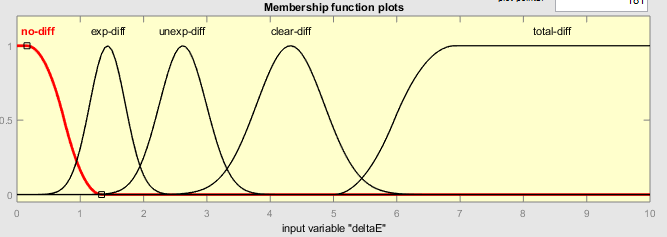
\includegraphics[scale=0.8]{images/rete2-membership-deltae.PNG}
\end{center}
\caption{Funzione di membership DeltaE (distanza euclidea)}
\label{fig:membdeltae}
\end{figure}

Per il colore (Hue) abbiamo utilizzato i range indicati nella tabella della figura \ref{fig:ciehue}\footnote{\url{https://www.researchgate.net/profile/Nele_Dael/publication/299491827/figure/fig6/AS:349601765838853@1460362964268/CIE-LCh-hue-categorization.png}}.
\begin{figure}[!ht]
\begin{center}
	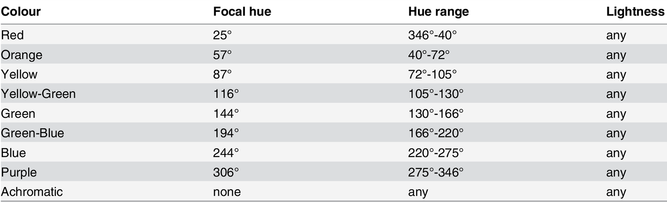
\includegraphics[scale=2.5]{images/CIE-LCh-hue-categorization.png}
\end{center}
\caption{Istogramma delle DeltaE delle coppie (master, copia disturbata)}
\label{fig:ciehue}
\end{figure}

\begin{figure}[!ht]
\begin{center}
	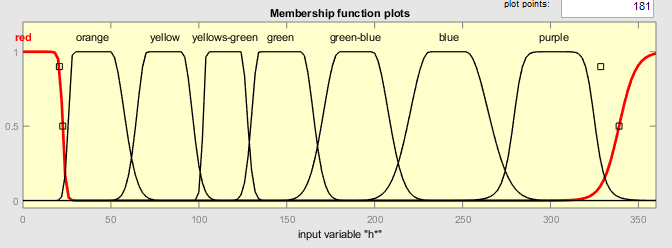
\includegraphics[scale=0.8]{images/rete2-membership-colors.PNG}
\end{center}
\caption{Funzione di membership Hue (Colore)}
\label{fig:membcolor}
\end{figure}

\begin{figure}[!ht]
\begin{center}
	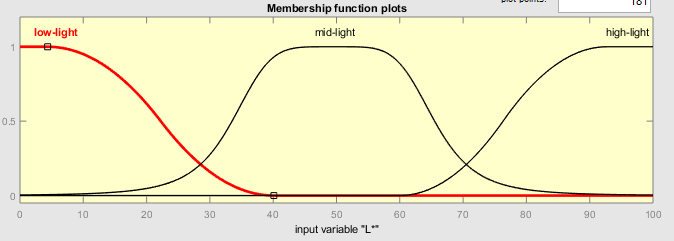
\includegraphics[scale=0.8]{images/rete2-membership-light.PNG}
\end{center}
\caption{Funzione di membership Light}
\label{fig:memblight}
\end{figure}

\begin{figure}[!ht]
\begin{center}
	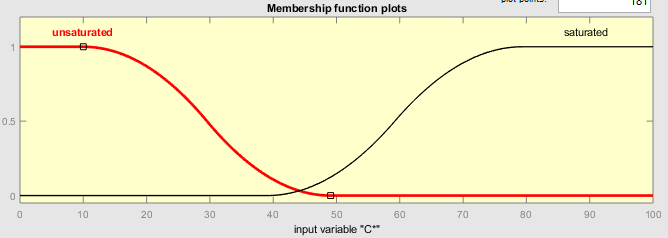
\includegraphics[scale=0.8]{images/rete2-membership-saturation.PNG}
\end{center}
\caption{Funzione di membership Saturation}
\label{fig:membsaturation}
\end{figure}

\section{Regole}
In base alle zone dello spazio LCh che abbiamo elencato prima, mostriamo le regole inserite nella rete Mamdani per la correzione dei DeltaE:
\begin{table*}[!ht]
\centering
\begin{tabular}{|c c c c c c |}
\hline
L & c  & h & $\Delta E_{orig}$ & $\Delta E_{adj}$ & peso\\ \hline
-  & -           & -          & total-diff        & total-diff   & 0.2 \\ \hline
-  & -           & -          & clear-diff        & clear-diff   & 0.2 \\ \hline
-  & -           & -          & unexp-diff        & unexp-diff   & 0.2 \\ \hline
-  & -           & -          & exp-diff          & exp-diff   & 0.2 \\ \hline
-  & -           & -          & no-diff          & no-diff   & 0.2 \\ \hline
low-light  & -           & -          & total-diff        & exp-diff   & 1 \\ \hline
low-light  & -           & -          & clear-diff        & exp-diff   & 1 \\ \hline
low-light  & -           & -          & unexp-diff        & no-diff   & 1 \\ \hline
low-light  & -           & -          & exp-diff          & no-diff   & 1 \\ \hline
mid-light  & saturated   & orange     & unexp-diff        & exp-diff   & 1 \\ \hline
mid-light  & saturated   & green      & unexp-diff        & exp-diff   & 1 \\ \hline
mid-light  & saturated   & green      & exp-diff          & no-diff   & 1 \\ \hline
mid-light  & saturated   & blue       & clear-diff        & exp-diff   & 1 \\ \hline
high-light & saturated   & yellow     & unexp-diff        & no-diff   & 1 \\ \hline
high-light & saturated   & yellow     & clear-diff        & exp-diff   & 1 \\ \hline
not(low-light) & unsaturated & -      & not(no-diff)      & exp-diff   & 1 \\ \hline
not(low-light) & unsaturated & -      & no-diff           & no-diff   & 1 \\ \hline
\end{tabular}
\caption{Regole di inferenza del sistema Madamani}
\label{tab:rules}
\end{table*}

\section{Risultati}
Quello che ci aspettavamo, con l'implementazione della rete, era una differente distribuzione dei DeltaE corretti rispetto a quelli iniziali: questo risultato è confermabile guardando gli istogrammmi in figura \ref{fig:fuzzyhistogramcomparision}. Le operazioni di fuzzyfication e defuzzyfication hanno concentrato, maggiormente, i DeltaE nelle zone specificate dalla funzione di membership e dalle regole di inferenza inserite.
\begin{figure}[!ht]
\begin{center}
	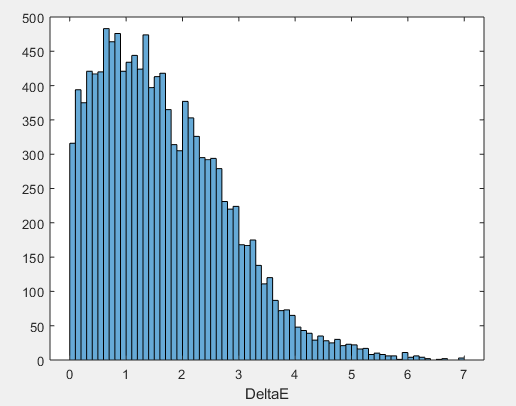
\includegraphics[scale=0.545]{images/fuzzy-istogramma1.PNG}
	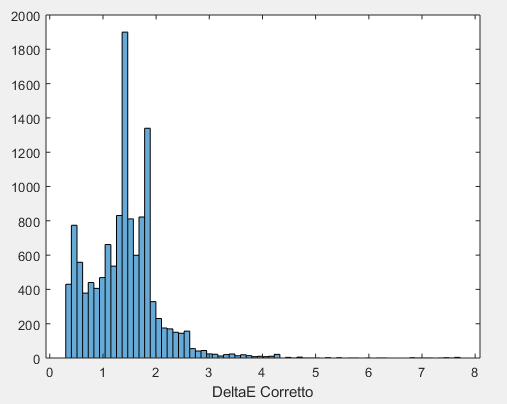
\includegraphics[scale=0.545]{images/fuzzy-istogramma2.PNG}
\end{center}
\caption{Comparazione Istogrammi DeltaE Originali / DeltaE Corretti}
\label{fig:fuzzyhistogramcomparision}
\end{figure}

\subsection{Risultati Rete Neurale}
L'utilizzo dei DeltaE corretti per il training di una nuova rete neurale ha scaturito la necessità di estrarre e selezionare, nuovamente, le feature. In particolare le nuove feature estratte sono state:
\\\\
\textbf{master}: var(1), median(1), median(3), skewness(5), maxYValue(2), indexAtMaxY(1)
\\
\textbf{copy}: median(1), median(3), skewness(1), skewness(5), maxYValue(2), indexAtMaxY(2)

Estraendo 12 feature e utilizzando 10 neuroni nell'hidden layer (1 layer), abbiamo riscontrato:
\[Mean\ Squared\ Error \simeq 0.0395, R \simeq 0.954\]

Le performance della rete sono peggiorate, a parità di numero di feature e neuroni dello strato nascosto. Questo è imputabile al fatto che la rete fuzzy rende più complesso il legame tra i colori in ingresso e le distanze calcolate: nel primo caso la distanza era euclidea, nel secondo caso è modificata secondo le regole della rete fuzzy (quindi è una funzione più complessa per il fitting).

L'aumento del numero delle feature non aumenta in maniera significativa il valore dell'MSE o del coefficiente R, quindi consideriamo 12 feature (e 10 neuroni) come il miglior compromesso tra complessità e prestazioni della rete. Il Mean Squared Error risulta essere di tre ordini più piccolo rispetto al massimo valore di DeltaE previsto, cioè 10, quindi può essere considerato accettabile.

\begin{figure}[!ht]
\begin{center}
	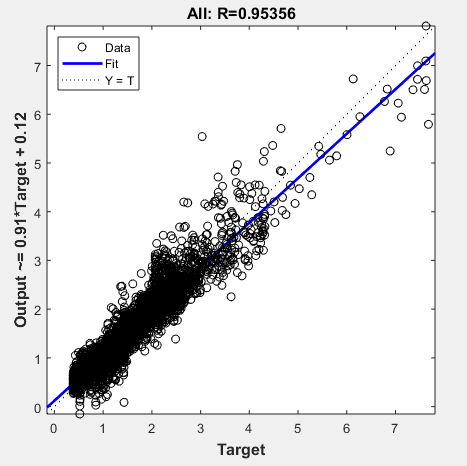
\includegraphics[scale=1]{images/rete2-regression.PNG}
\end{center}
\caption{Retta di Regressione della rete neurale, dopo l'introduzione dei DeltaE corretti}
\end{figure}